\documentclass[preprint,12pt]{elsarticle}
\journal{Future Generation Computer Networks}
\usepackage{amsmath, amsthm, amssymb,  graphicx}
\usepackage{subfigure}
%\usepackage{subfig}
%\usepackage{cite,citesort}
%\usepackage{cite}
\usepackage{multirow}
\usepackage{epsfig}
%\usepackage{epstopdf}
%\usepackage{algorithmic}
\usepackage{algorithm2e}

\usepackage{url}

% *** SPECIALIZED LIST PACKAGES ***
%
%\usepackage{algorithmic, algorithm}
\begin{document}

\begin{frontmatter}

%% Title, authors and addresses

%% use the tnoteref command within \title for footnotes;
%% use the tnotetext command for the associated footnote;
%% use the fnref command within \author or \address for footnotes;
%% use the fntext command for the associated footnote;
%% use the corref command within \author for corresponding author footnotes;
%% use the cortext command for the associated footnote;
%% use the ead command for the email address,
%% and the form \ead[url] for the home page:
%%
%% \title{Title\tnoteref{label1}}
%% \tnotetext[label1]{}
%% \author{Name\corref{cor1}\fnref{label2}}
%% \ead{email address}
%% \ead[url]{home page}
%% \fntext[label2]{}
%% \cortext[cor1]{}
%% \address{Address\fnref{label3}}
%% \fntext[label3]{}

\title{Low-Carb: A Practical Technique for Improving Energy Efficiency in Operational Cellular Networks}

%% use optional labels to link authors explicitly to addresses:
%% \author[label1,label2]{<author name>}
%% \address[label1]{<address>}
%% \address[label2]{<address>}

\author[LUMS]{Muhammad Saqib Ilyas\corref{cor1}}
\cortext[cor1]{Corresponding author}
\author[LUMS]{Ghufran Baig}
\author[LUMS]{Zartash Afzal Uzmi}
\author[LUMS]{Ihsan Ayub Qazi}
\author[WaridTel]{Bilal Rassool}
\address[LUMS]{\ead{\{saqibm, 000000, zartash, ihsan.qazi\}@lums.edu.pk}School of Science and Engineering, LUMS, Lahore, Pakistan}
\address[WaridTel]{\ead{bilal.rassool@waridtel.com}Warid Telecom, Lahore, Pakistan}



\input{Sections/Abstract}
\begin{keyword}
%% keywords here, in the form: keyword \sep keyword

%% MSC codes here, in the form: \MSC code \sep code
%% or \MSC[2008] code \sep code (2000 is the default)
Green communication, BTS power-saving, energy conservation, energy efficiency
\end{keyword}

\end{frontmatter}

%%
%% Start line numbering here if you want
%%
% \linenumbers

%% main text
\section{Introduction}
\label{sec:intro} Intro bro~\cite{Chabarek08powerawareness}

\section{Related Work}
\label{sec:related}

\section{Problem Formulation}
\label{sec:formulation}
\subsection{Single Base Transceiver Station (BTS)}
Power consumed by a BTS, as a function of traffic load, can be
well approximated as a linear curve with a non-zero
y-intercept~\cite{Peng:2011:BTSSaving:Mobicom} given as
$P_1+l(P_2-P_1)/t_{max}$. Here $P_1$ and $P_2$ are the power
consumption at no load and full load, respectively, $l$ is the
number of calls presently being handled, and $t_{max}$ is the
maximum number of calls that can be handled.

Let $\delta$ be the traffic threshold at which the \textit{BTS
power savings} is applied (i.e., when BTS deactivates some TRXs
moving into low-power mode). Since all TRXs are identical, the
per call increase in power consumption, and hence the slope of
the power consumption profile in Fig.~\ref{fig:powermodel},
remains the same whether or not some TRXs are deactivated. As
also indicated in Fig.~\ref{fig:powermodel}, the no-load power
consumption drops to $P_1-\gamma$ in the low-power mode, where
$\gamma$ is a constant that depends on the equipment type and
the number of TRXs deactivated.

If $x$ is an indicator variable which is 1 when \textit{BTS
power savings} is applied, and $0$ otherwise, then the BTS
power consumption may be given by $P_1+l(P_2-P_1)/t_{max} -
(1-x)\gamma$, also indicated in Fig.~\ref{fig:powermodel} by
the piecewise linear solid line.

\begin{figure}
\centering
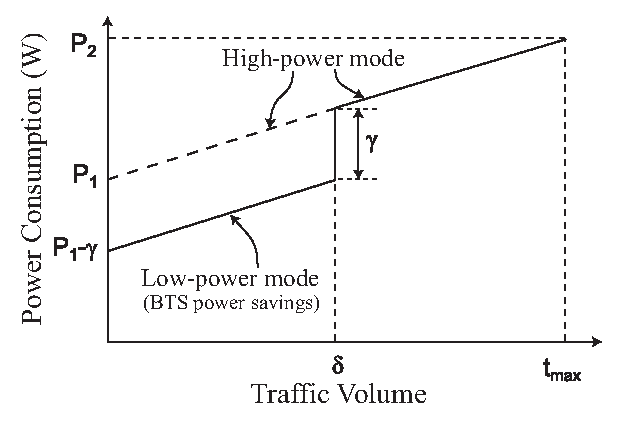
\includegraphics[width=0.28\textwidth]{figures/powermodel.eps}
\caption{BTS power consumption model. Low-power (BTS power savings) mode is optional and kicks in at low loads.}
\label{fig:powermodel}
\end{figure}

\subsection{Multi-BTS Cellular Setting}
Consider an area with $n$ active callers being served by $m$ BTSs.
We introduce indicator variable $w_{i,j}$, which is $1$ if call
$i$ \textit{is being} handled at BTS $j$ and $0$ otherwise. We
assume availability of an $n\times m$ matrix whose entry
$c_{i,j}$ is $1$ if caller $i$ \textit{can be} served through
BTS $j$ without exceeding the uplink or downlink budgets.
This information can be extracted by the data periodically
transmitted by each MS comprising the received signal strength
from nearby BTSs during a call. We also introduce indicator
variable $x_j$, which is $1$ if BTS $j$ is operating in
high-power mode (i.e., without \textit{BTS power savings}) and
$0$ otherwise. Using these variables and parameters, we can
formulate an optimization problem to minimize the total power
consumption over the network as:
\begin{align}
\textit{minimize} \quad \sum_{j=1}^{m} \left[
P_1+\sum_{i=1}^{n}\frac{w_{i,j}(P_2-P_1)}{t_{max}}-(1-x_j)\gamma
\right]
\end{align}
subject to the following constraints:
\begin{align}
& \sum_{j=1}^m w_{i,j} = 1 \qquad \forall i \\
& w_{i,j} \leq c_{i,j} \qquad \forall i, j \\
& \sum_{i=1}^nw_{i,j}-\delta \leq Mx_j \qquad \forall j%\\
\end{align}
\begin{align}
& \sum_{i=1}^n w_{i,j} \le t_{max} \qquad \forall i \\
%\end{align}
%\begin{align}
& w_{i,j}, x_j \in {0,1} \qquad \forall i, j%\\
%x_j \in {0,1}
\end{align}

The objective function is a simple generalization from the case
of one BTS. The first constraint ensures that no active call is
dropped just to save on power. The second constraint secures
the uplink budget by ensuring that no call is routed to a BTS
that can not handle it. The third constraint picks the correct
value for the decision variable $x_j$. The fourth constraint is the capacity constraint on all BTSs, while the last
constraint is the binary value constraint on the decision
variables.

The above optimization problem is a Binary Integer Program
(BIP), which is NP-Hard. It is intractable to solve it for an
operator's entire network, but solving it for a subset of the
network will provide some estimates of the amount of energy
savings possible using Low-Carb. Deployment to large operator
networks would require approximation algorithms.
\section{Experimental Setup}
\label{sec:expermintalsetup}
Our dataset is obtained from a cluster of 26 BTSs operated by a large network operator with more than 7000 sites. These sites are spread over a $31.25$ $km^2$ urban terrain. We obtained each site's coverage prediction using a tool popular amongst the operators called Forsk Atoll. With this information, alongwith a caller's location, we can determine the candidate set of BTSs for the corresponding call (the $c_i^j$ parameters). Note that in this work, we do not incorporate user mobility into our model, since we are only interested in instantaneous optimization.

Also available to us are the hourly cumulative traffic, in Erlang, for each of the sites, spanning two consecutive weekdays. The traffic remained remarkably similar across both days for each site. We have, therefore, only used one day's traffic data in our experiments.

Using the above datasets, we conducted a set of experiments mimicking a 24-hour operation of a subset of a cellular network. Each experiment is a discrete event simulation of the arrival and placement of calls. Since our dataset does not include the arrival times and duration of calls, we synthetically generated this information using the assumption of Poisson call arrivals and exponentially distributed call duration with a mean of $180$ seconds~\cite{Gerla:1995:MMM:276418.276421}.

For every hour, the simulator determines the Poisson call arrival rate for each BTS, using Little's Law and the BTSs traffic intensity for that hour. Using the resulting Poisson process, calls are generated such that it is equally likely for a call to be anywhere in the serving BTSs coverage area.

Our simulator tracks the call volume at every BTS on a minute's granularity. This enables us to calculate the power consumption level (in Watts) of the BTS during each minute. Accumulating these numbers over the 24 hour period leads to the daily amount of energy consumed (in kWh) if no optimization is used in the network. Our simulator also monitors each BTSs call volume every minute and places the ones with sufficiently low traffic into power-saving mode. This enables us to calculate the possible energy savings using BTS power-saving feature. In addition, our simulator also periodically determines the instantaneous optimal call placement configuration that minimizes the power consumption level by handing-off some calls, thereby placing a maximal number of BTSs in power-saving mode. This allows us to determine the energy savings possible by combining call hand-offs with BTS power-saving.

%In order to evaluate Low-Carb's effectiveness, we conducted simulation experiments over a set of 26 BTSs spread over a $31.25$ $km^2$ area in an urban setting. These sites belong to a large cellular operator with more than 7000 sites. For each of these sites, we obtained hourly cumulative voice traffic (in Erlangs) for two consecutive weekdays. Since the traffic for both days was remarkably similar on all sites, we have reported results of experiments utilizing just a 24 hour traffic trace.
%
%Our experiments consist of a discrete event simulation of call arrivals, placement and then possible hand-offs, driven by real traffic traces. Since the traffic traces do not include call arrival times and distributions, we simulate call arrivals and departures using the assumption of Poisson call arrivals with a mean call duration of $180$ seconds~\cite{Gerla:1995:MMM:276418.276421}. For a given hour, the Poisson call arrival rate is determined for each BTS separately, through Little's Law, by substituting the mean call duration and the corresponding traffic intensity. A new call is equally likely to be anywhere in it's serving BTSs coverage area. For our simulations, we used coverage predictions from a commercial tool Forsk Atoll.
%
%Having simulated call arrivals and associations with serving BTSs, our simulator continuously determines the BTSs with sufficiently low traffic and puts them in power-saving mode. Similarly, when the traffic rises above this threshold, the BTSs are brought out of power-saving mode. This allows us to determine the savings achievable using BTS power-saving alone. Furthermore, we periodically determine the instantaneous optimal mapping of the current set of active calls to the BTSs such that a maximal number of BTSs can be put in power-saving mode. Between two successive optimizations, new calls are associated with the BTS from which the caller receives the best signal, with no regard to optimality. The energy saving thus obtained would help us determine the utility of combining call hand-off with BTS power-saving.

The call placement re-optimization may be done at various frequencies. A very aggressive re-optimization regime would keep the network in an optimal state more often than a conservative one, thereby enabling greater energy savings. In order to study the scaling of energy saving with re-optimization frequency, we experimented with a range of intervals between successive optimizations, ranging from a minute to an hour. For a deployment, the re-optimization frequency that can be used would depend on the costs associated with each re-optimization. Let us now consider such costs.

First and foremost, a computational cost is incurred with each optimization. In our case, an optimization run to determine the optimal state over $26$ BTSs required an average running time of about $50$ seconds on a Core i3 laptop with 4 GB of RAM. An optimization requiring $50$ seconds would not be practical to use every minute but may be fine if used less often. For a practical deployment the computational time can be reduced by using a combination of a more powerful machine, distributed optimization and approximation algorithms. 

In addition to the computational overhead, for every unit of energy saved some extra energy may be consumed in the network to perform call hand-offs or entering and leaving BTS power-saving mode. Call hand-offs and TRX (de)activation involve signaling between a Base Station Controller (BSC), BTSs and MSs. The additional energy incurred thus, should be small, because it has been observed that variation in power consumption of network equipment with changes in traffic volume (data or control) is quite small~\cite{Chabarek08powerawareness}. As far as increased power consumption on MSs due to a greater number of call hand-offs is concerned, we opine that it may be negligible because the MSs energy consumption is far outweighed by that of BTSs. %Presently, we do not have quantitative results to back this claim.

%Our dataset consists of the location of
%26 BTSs in an urban setting, scattered over an area of about $31.25$ $km^2$, from a large operator (with more
%than 7000 cell sites) and the corresponding hourly cumulative
%traffic traces for several days. We conducted simulation
%experiments using a 24 hour subset of the traffic traces only;
%the traffic data for other days (except for weekends) was
%remarkably similar. Data about individual call arrival times
%and durations was not available to us.
%%because it's collection would have a large storage impact at
%%the operator's end.
%Therefore, we synthetically generated the call arrival times
%and durations.
%
%%assuming Poisson arrivals and a negative-exponential
%%distribution of call durations with a mean value of $180$
%%seconds~\cite{Gerla:1995:MMM:276418.276421}. The Poisson
%%arrival rate for each hour is obtained from Little's law by
%%using the corresponding traffic volume and average call
%%duration.
%
%We developed a discrete event simulator in Matlab that
%generates calls arrivals randomly according to Poisson arrival
%process while setting call duration according to an exponential
%distribution with mean of $180$
%seconds~\cite{Gerla:1995:MMM:276418.276421}. The Poisson
%arrival rate for each hour is obtained from Little's law by
%using the corresponding traffic volume and average call
%duration. Each call is at first associated with the BTS from
%which it receives the strongest signal. This establishes the
%benchmark for evaluation of our proposed scheme. Within the
%simulation, we periodically invoked the CPLEX optimizer and
%obtained the instantaneous mapping between calls and their
%corresponding serving BTSs. We experimented with varying
%frequency of re-optimization ranging from very aggressive
%(every minute!) to conservative with once per hour
%re-optimization. For each re-optimization interval, we
%determined the savings in energy consumption compared to the
%benchmark.
%
%To determine the possible set of serving BTSs for a given call,
%we have used a simple heuristic of a circular coverage area
%around a cell site approximated from the coverage predictions
%obtained through a commercial software, Forsk Atoll. Our
%procedure only requires availability of a 0-1 matrix
%representing this information and in practice a more accurate
%estimation technique may be plugged into our framework without
%requiring any changes.

%*** The following should change ***
% TODO to-do %

% Should we keep everything in the following para? or anything at all? Perhaps, the geographical size, yes... other info, your call Saqib! -Zartash

%BTSs come in different shapes and sizes. To obtain results that are applicable to most operators, we used three
%different models for BTS power consumption that we found in
%recent literature. These models are described next.

\subsection{Site Characteristics}
\label{subsec:sitetypes} All sites in our dataset had three sectors, each equipped with 6 TRXs, for a maximum of %In the GSM standard, each TRXs signal may be used by as many as $8$ voice/control channels thanks to Time Domain Multiple Access (TDMA). This means that each site is equipped with $3\times6\times8 = 144$ channels of which four in each sector were reserved for control and broadcast channels, resulting in each site having a traffic capacity ($t_{max}$) of $132$ simultaneous voice calls. 
%Each site is capable of handling 
132 simultaneous voice calls\footnote[1]{Each TRX's frequency is shared in time-domain  by 8 calls for  a total of $3\times6\times8=144$ channels. Four channels in each sector were reserved for control and broadcast purposes.}. The GSM standard includes a provision for half-rate calls, which enables handling greater traffic at the expense of reduced voice quality by allowing a single voice channel to be shared amongst two calls, each using a half-rate codec. In this paper, we only shuffle full-rate calls around, which may be, in reality, two half-rate calls. We do not foresee any significant error arising from using this convention.

We consider a scaling down from a $``6+6+6"$ site to a $``2+2+2"$ site, which means that $\delta$ should be strictly less than $t_{max}/3$ to avoid quick oscillations into and out of BTS power-saving mode due to short-term traffic variations. %when a BTS goes to low-power mode, it has some residual capacity on the remaining TRXs and unnecessary oscillations between low-power and high-power model are avoided. 
We have arbitrarily set $\delta$ equal to $\lceil t_{max}/3\rceil -5$, because $5$ seemed to be a good enough number compared to a sector's overall capacity and the typical utilization of a site in our datasets.

The BTS power consumption model parameters may vary from one BTS model to another. In this paper, we use three different sets of model parameters as listed in table~\ref{tab:models}. We now describe the sources and methods from which we obtained these models.
\subsubsection{Model 1}
\label{subsubsec:model1}For the first model, we have used $1.5kW$ as the maximum power consumption~\cite{mbakwe:btshybribpower:2011:necec}, a $20W$ per TRX saving when scaling the BTS down~\cite{flexibsc} and a $5\%$ swing in power consumption between no-load and full-load~\cite{Peng:2011:BTSSaving:Mobicom}.

\subsubsection{Model 2}
\label{subsubsec:model2} Lorincz et. al reported the single sector DC power consumption for a GSM 900 BTS~\cite{Lorincz:BTS-Measure:Sensors:2012}. The sector under consideration had 7 TRXs, as opposed to 6 TRXs in our case. To approximate the DC power consumption for a site with 3 sectors, each with 6 TRXs, we scaled the power consumption by a factor of $3\times6/7$. The DC power consumption does not include the AC power consumed in the power supply units and in air-conditioning. We must, therefore, also compensate for those, to obtain the overall site power consumption. Power supply unit load is negligible compared to air-conditioning, which has a typical power consumption of 1 kW~\cite{mbakwe:btshybribpower:2011:necec}. We applied this scaling and addition to the minimum reported DC power consumption for the GSM 900 site to obtain an approximate value of $P_1$ for a site comparable to ours. Similarly, we used the maximum reported DC power consumption and applied the scaling and AC load correction to approximate the value of $P_2$. Furthermore, the authors measured a drop of $50W$ in power consumption when a TRX is disable, which gives us the value of $\gamma$ as listed in table~\ref{tab:models}.

%For the second model, we picked the measurements for the GSM 900 BTS in~\cite{Lorincz:BTS-Measure:Sensors:2012}. The minimum and maximum reported power consumption for a sector with $7$ TRXs at this BTS were $517.6W$ and $1012.5W$ respectively. For a sector with $6$ TRXs, as in our case, the minimum and maximum power consumption would be (roughly) $467.6W$ and $962.5W$ respectively. For a site with three such sectors, the overall minimum and maximum power consumption would be three folds, i.e., $1401.8W$ and $2887.5W$ respectively. This is the DC power consumption as reported in~\cite{Lorincz:BTS-Measure:Sensors:2012}, which does not include the power consumed in air-conditioning and power supply units. The latter consume negligible power as compared to the former, which is typically $1kW$~\cite{mbakwe:btshybribpower:2011:necec}. Therefore, under this model, we consider a site's minimum and maximum power consumption as $2401.8W$ and $3887.5W$ respectively. Also recall, that in case of the GSM 900 BTS,~\cite{Lorincz:BTS-Measure:Sensors:2012} reports a cut of $50W$ in power consumption when a TRX is deactivated.

\subsubsection{Model 3}
\label{subsubsec:model3}Using the same method as for model 2 in~\ref{subsubsec:model2}, we derived the values for $P_1$ and $P_2$ using the measurements for the GSM 1800 BTS in~\cite{Lorincz:BTS-Measure:Sensors:2012}. As for the value of $\gamma$, the paper reported a $100W$ cut in power consumption when deactivating a single TRX. The parameter values for this model are given in Table~\ref{tab:models}

\begin{table}
\centering
\begin{tabular}{|c|c|c|c|}
\hline
Parameter & \multicolumn{3}{|c|} {Value} \\
\cline{2-4} \ & Model 1 & Model 2 & Model 3 \\
\hline $P_1$ & 1425 & 2401.8 & 2341.5 \\
\hline $P_2$ & 1500 & 3887.5 & 2973.9 \\
\hline $\gamma$ & 20 & 50 & 100 \\
\hline
\end{tabular}
\caption{BTS model parameter values}
\label{tab:models}
\end{table}

\section{Results}
\label{sec:results}
The following results were obtained through simulation experiments driven by real traffic traces and deployment geography. The experiments perform a combination of activation of BTS power-saving mode on BTSs alongwith a periodic update of serving BTS for each active call, such that the instantaneous energy consumption in the network is minimized.

First, we consider the benefit of BTS power-saving alone, resulting from traffic diversity at each BTS compared to running the network in the default configuration. The percentage reduction in energy consumption is listed in table~\ref{tab:psonly}. The results indicate that a saving of between 4\% and 12\% can be achieved in a network just by activating BTS power savings. We note here that some of these results are in agreement with Ericsson's claim of saving 10-20\% energy by using BTS power-saving on Germany's Vodafone network~\cite{ericssonclaim}. 

In absolute terms, this represents a cumulative saving of between 43 kWh and 217 kWh per day on 26 BTSs. Now, consider that there are five cellular oeprators in Pakistan: Mobilink with more than 8500 sites~\cite{mobilinksitecount}, Ufone with more than 8000 sites~\cite{ptaannreport}, Zong with more than 5500 sites~\cite{ptaannreport}, Telenor with more than 7000 sites~\cite{telenorsitecount} and Warid with more than 4500 sites~\cite{ptaannreport}. Overall, there were more than 31000 sites in Pakistan at the end of 2011. We extrapolated the daily energy savings number over 26 BTSs to calculate the daily energy savings possible for a country like Pakistan with over 31000 BTSs (see the last row of table~\ref{tab:psonly}). The results indicate that mere activation of BTS power saving option itself can save quite a bit of electrical energy, a critical resource, especially in a developing country. As we shall see next, greater energy savings are possible if we couple periodical call shuffling with BTS power savings in the network. 

\begin{table}
\centering
\begin{tabular}{|c|c|c|c|}
\hline Energy saving & Model 1 & Model 2 & Model 3 \\
\hline Percentage & 4.73\% & 5.43\% & 12.89\% \\
\hline Daily absolute saving & 43.28 & 109.68 & 217.12 \\
over 26 BTSs (in kWh) & \ & \ & \ \\
\hline Country-wide daily saving & 51.6 & 130.77 & 258.87\\
over 31000 sites (in MWh) & \ & \ & \ \\
\hline
\end{tabular}
\caption{Energy savings by using BTS power savings only}
\label{tab:psonly}
\end{table}


If periodic optimization of call placement is coupled with BTS power-saving, the energy saving improves, as shown in Fig.~\ref{fig:results2}.
%As noted earlier, we expect to achieve greater energy savings by periodically handing-off calls from busier BTSs to nearby BTSs with lower traffic to put a maximal number of BTSs in power-saving mode. If the periodic re-optimization is done aggressively, the network would remain in a nearly optimal state more often. On the other hand, a less aggressive policy would have the network in a nearly optimal state less often. We, therefore, expect that savings in power consumption should increase when the interval between re-optimization episodes is decreased. Since we are interested in the overall impact of the power saving scheme, the percentage power savings are computed over the entire network and not per BTS. %Furthermore, the percentage savings are computed over the default mapping of calls to BTSs, i.e., each call is associated with the BTS that the caller receives the strongest radio signal from.
%
%The percentage reduction achieved by using Low-Carb for the three BTS models is plotted in Fig.~\ref{fig:results2}. 
For all three BTS models, we see an almost linear increase in power saving as the duration of the re-optimization interval is decreased. Recall that the three models are significantly different in terms of power consumption (see Table~\ref{tab:models}). We can not directly say that because model 3 BTS offers the highest percentage reduction in energy consumption, it also saves the most energy (in kWh). %The results in Fig.~\ref{fig:results2} are quite useful to study the sensitivity of Low-Carb to the duration of re-optimization interval. However, one can't compare the three BTS models based on that, because the power consumption profiles are different for the three. For instance, a $15\%$ saving on $100kWh$ is not the same as a $15\%$ power saving on $500kWh$.

%\begin{figure}
%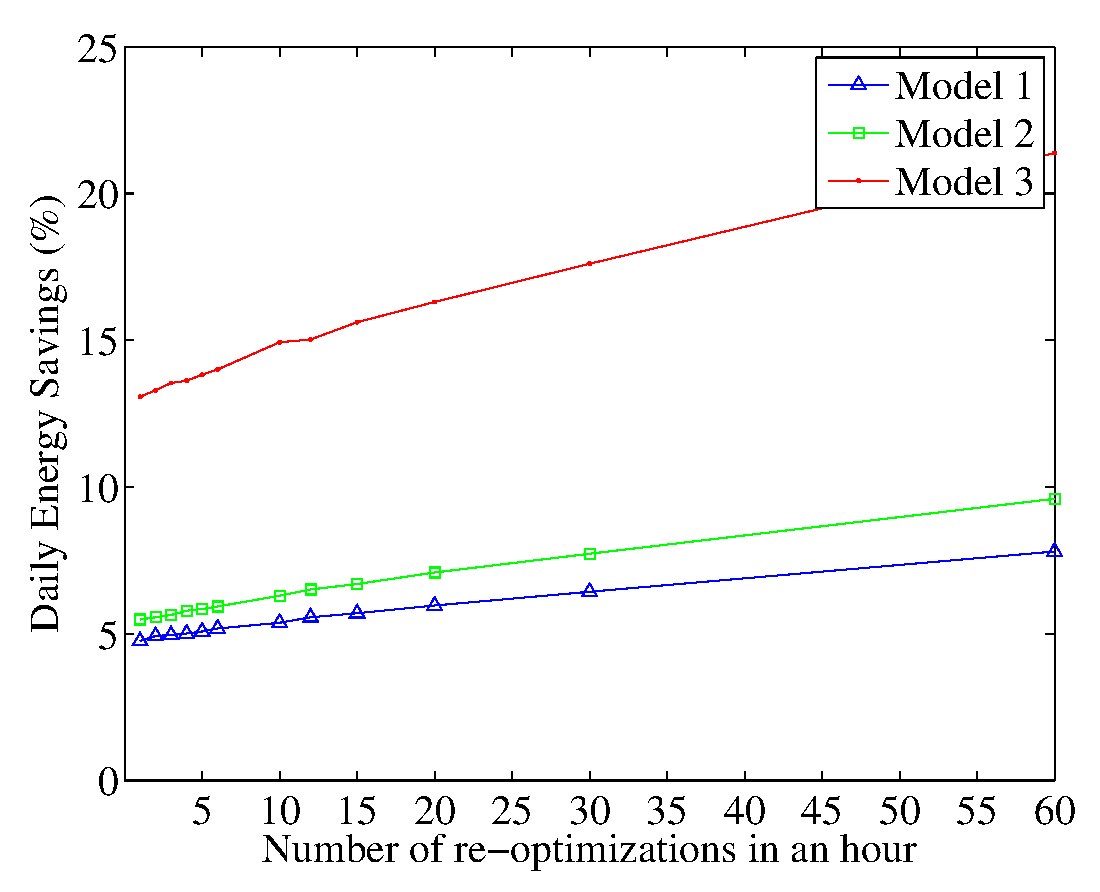
\includegraphics[width=0.5\textwidth]{figures/percent.savings.powersaving.eps}
%\caption{Percentage reduction in power consumption vs re-optimization interval - BTS Power Saving only}
%\label{fig:results1}
%\end{figure}

\begin{figure}
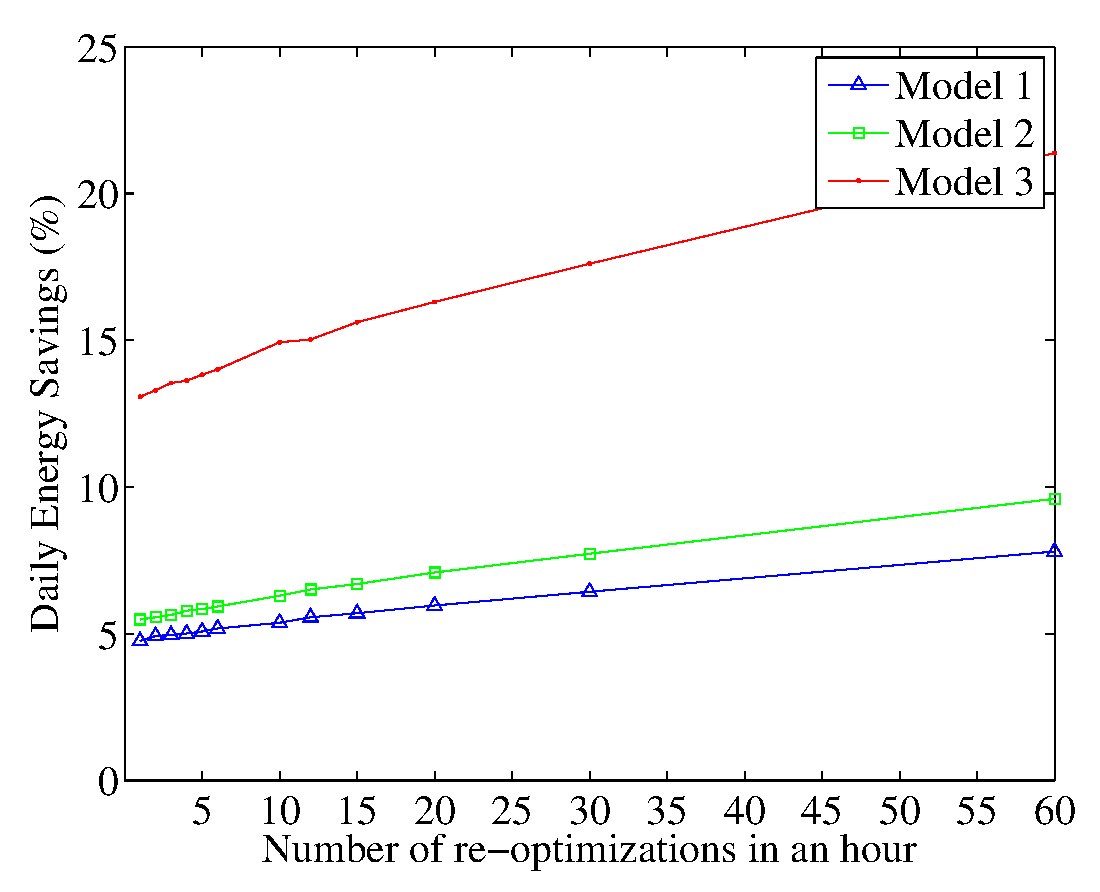
\includegraphics[width=0.45\textwidth]{figures/percent.savings.powersaving.eps}
\caption{Percent reduction in energy consumption vs re-optimization interval}
\label{fig:results2}
\end{figure}

%\begin{figure}
%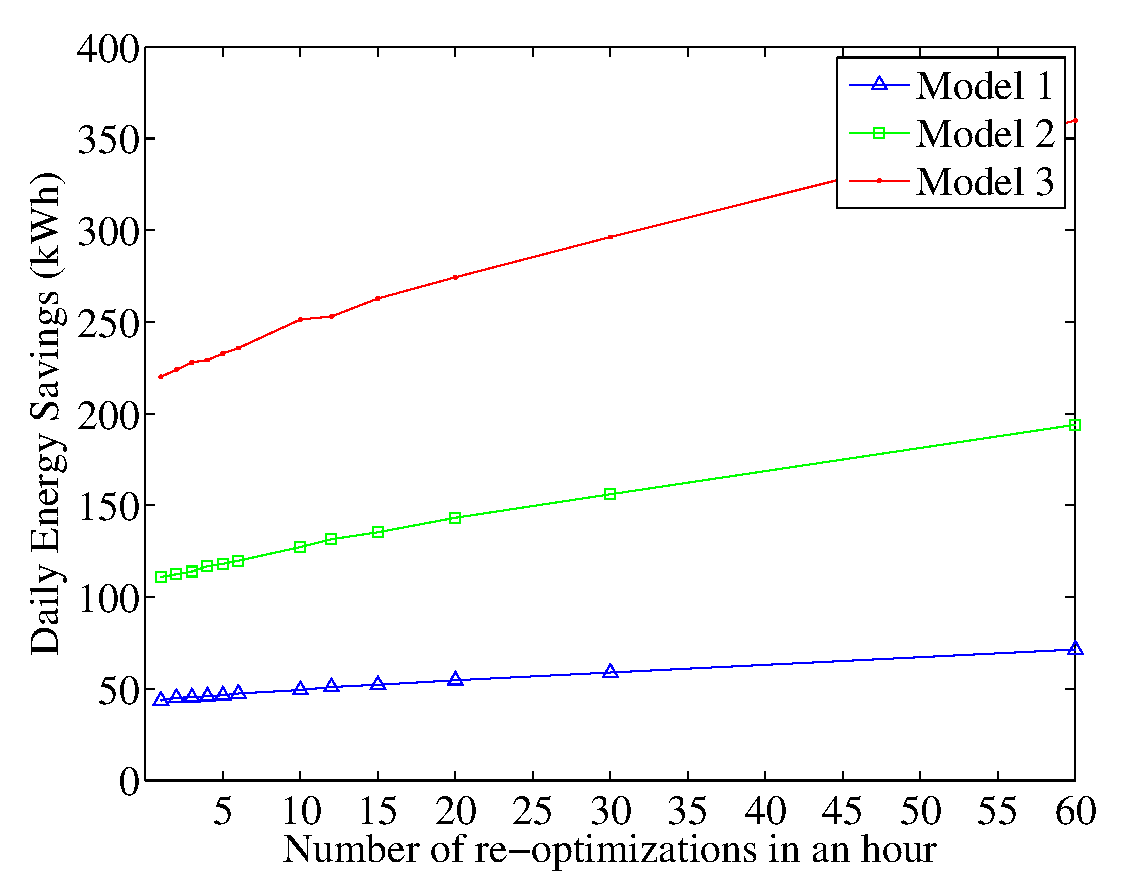
\includegraphics[width=0.5\textwidth]{figures/e.savings.powersaving.eps}
%\caption{Reduction in energy consumption through BTS Power Saving}
%\label{fig:results3}
%\end{figure}

To \textit{compare} the three BTS models in terms of energy saving potential, we also present the absolute reduction in energy consumption for the three BTS models in Fig.~\ref{fig:results4}. We see the same linear trend alongwith the same relative order of the three models in terms of amount of saved energy, as in Fig.~\ref{fig:results2}. 

Re-optimizing at an interval less than the mean call duration should offer greater savings than a less frequent re-optimization, because the former regime has the opportunity to optimize more by handing off most of the calls. This is confirmed in our results. For instance, for model 1 BTS, the gain in energy savings going from a 60 minutes inter-optimization interval to 30 minutes gains an energy saving of only 0.0506 kWh per minute, while decreasing the inter-optimization interval from 2 minutes to 1 minute gains 12.5421 kWh. %We notice a more pronounced separation between the three models in Fig.~\ref{fig:results4}, resulting from the considerable difference between the maximum and minimum power consumption levels for the three models, as well as the values of $\gamma$.

\begin{figure}
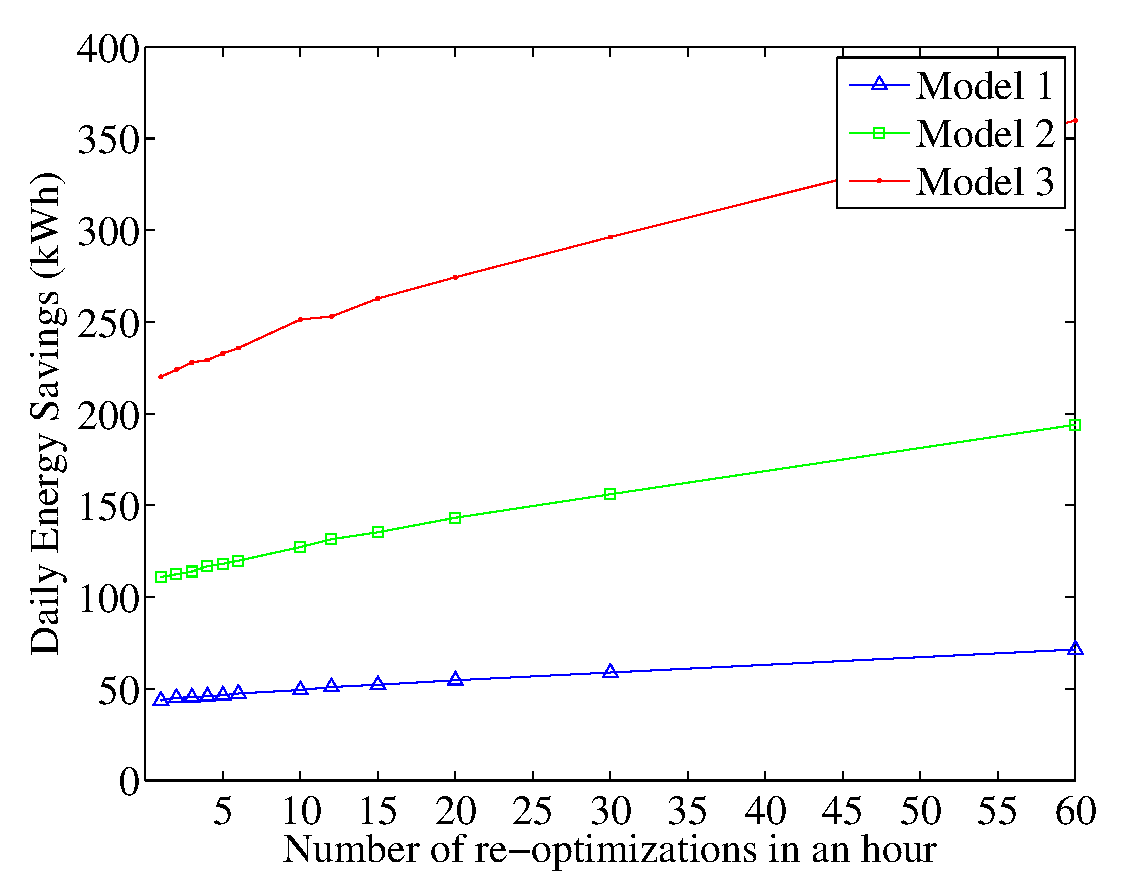
\includegraphics[width=0.45\textwidth]{figures/e.savings.powersaving.eps}
\caption{Reduction in energy consumption vs re-optimization interval}
\label{fig:results4}
\end{figure}

Let us now interpret what these results mean physically in terms of ecological impact. If we extrapolate our results, the total energy saving for Pakistan are projected to be $60.72$ MWh, $156.84$ MWh and $301.61$ MWh daily, respectively, according to the three BTS models. These savings in energy are significant, especially for small and developing countries. Since network deployments and traffic patterns are similar in different countries, we also expect that similar savings should be achievable in many other countries as well.

In the above extrapolation, we have assumed that the same amount of energy saving would be applicable in rural as well as urban settings. While this may not necessarily be true because the deployments are sparse in rural settings, resulting in reduced potential to save energy by means of call hand-off to neighboring sites, the potential to save energy merely by BTS power-saving should be higher in a rural setting because traffic loads are typically lower.
%An assumption in the above extrapolation is that the same amount of energy can be saved anywhere in the network. However, traffic patterns and deployment denisty vary in a given network. For instance, cellular networks in rural areas are typically characterized by lower traffic alongwith sparse deployments and, therefore, may not offer as much energy saving possibility as an urban setting (our dataset is for an urban setting). We do not expect that there would be no opportunity for energy savings in rural settings, because of multiple factors. This is partially correct because saving more energy by call-handoff is tough due to sparse deployments. However, the traffic is typically low in such areas, so there should be a greater opportunity to deactivate TRXs most of the time, resulting in greater savings in rural areas than urban. In an extended version of this paper, we will experiment with a dataset from a live network in a rural setting to assess the overall savings possible in a country-wide network.

%\begin{figure}
%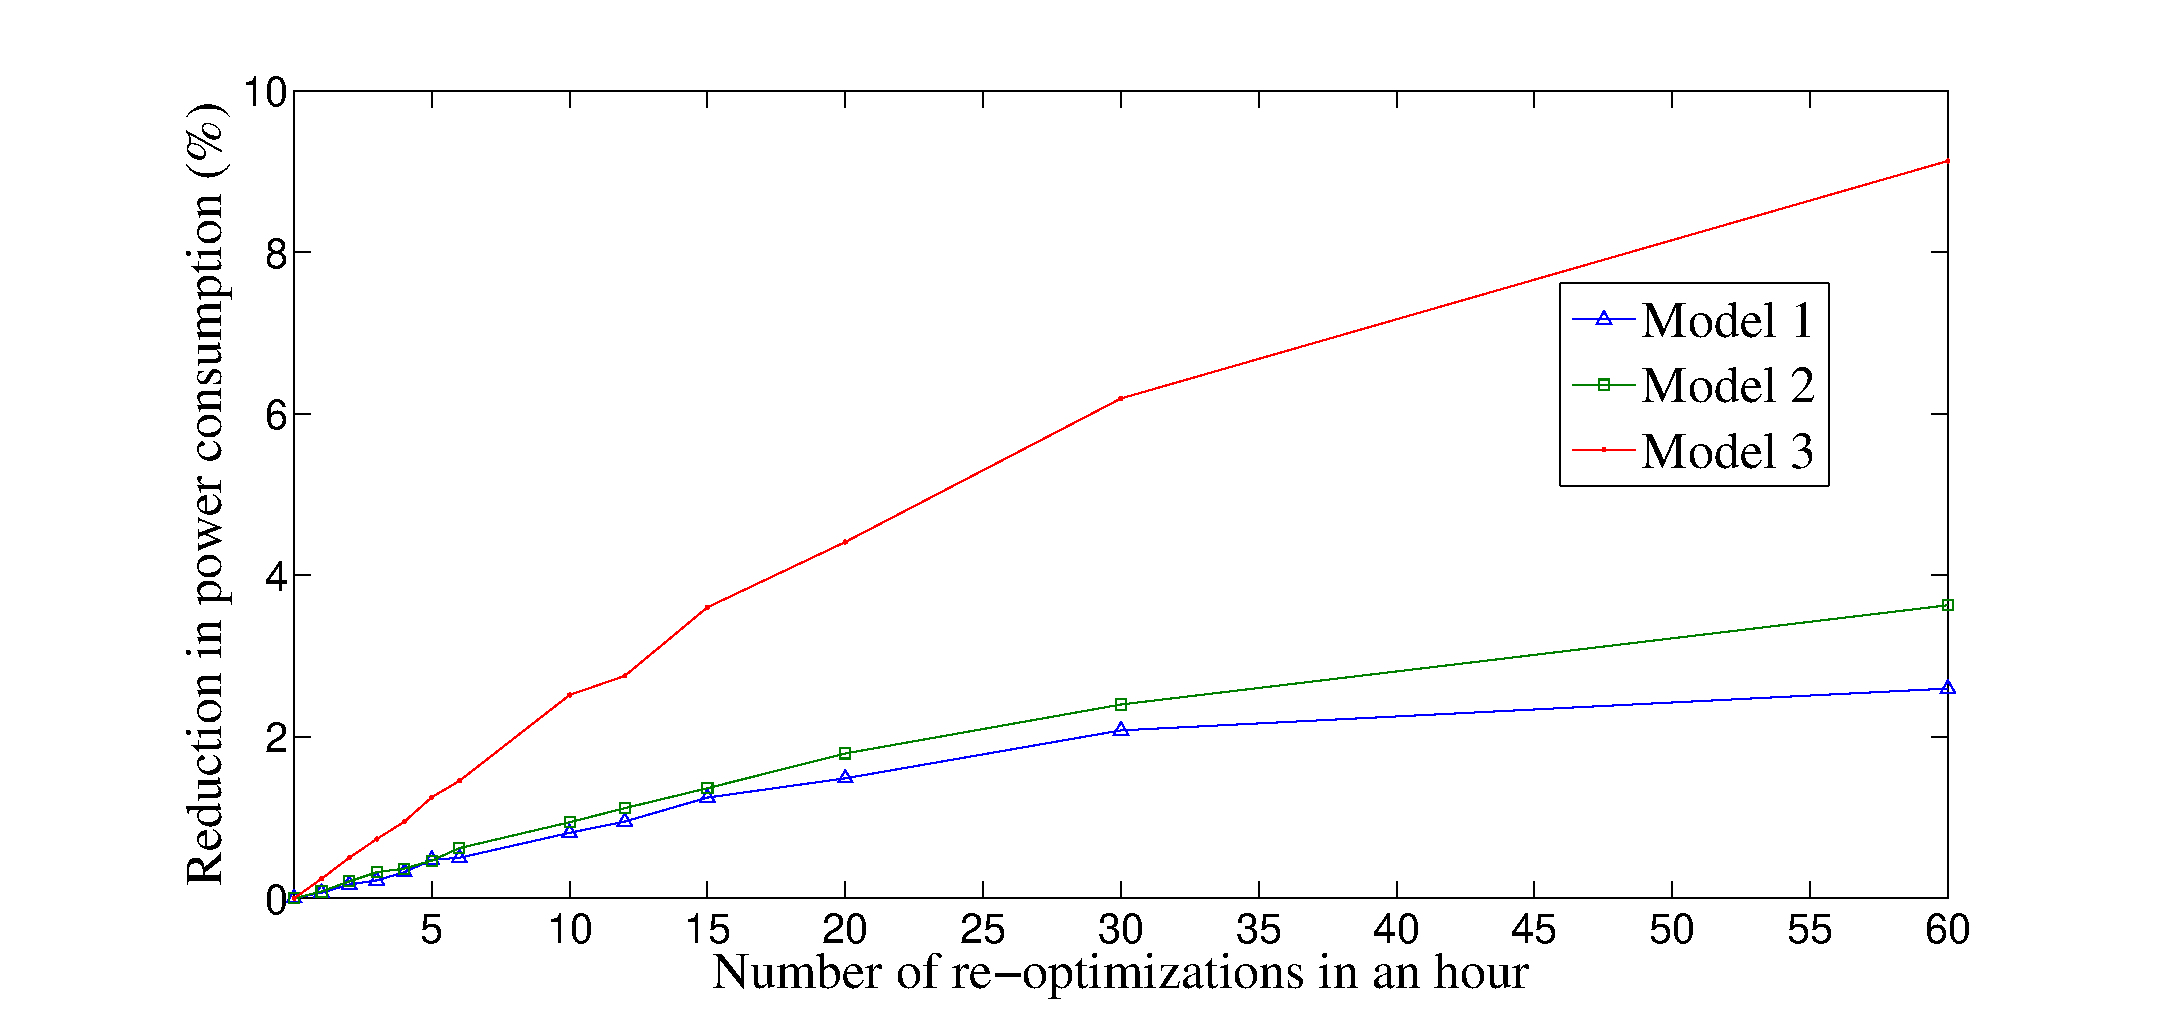
\includegraphics[width=0.5\textwidth]{figures/improvementplot.eps}
%\caption{Percentage reduction in power consumption vs re-optimization interval - Sparse deployment of $9$ BTSs}
%\label{fig:results1}
%\end{figure}
%
%For a region with sparse deployments, we plot the percentage savings in power consumption as the re-optimization interval was varied, in Fig.~\ref{fig:results1}. For model 1 BTS, we were only able to reduce the power consumption by about $2.5\%$ even if we re-optimized once every minute. This is expected because placing a BTS in power saving mode affords a saving of $240W$ (the value of $\gamma$), which is a small percentage of the maximum power consumption($1500W$) and this small saving is applicable only while the traffic at a BTS is below $\delta$.
%
%The percentage savings for model 2 BTS are somewhat better than those for the model 1 BTS. This would be due to the value of  $\gamma$ being a larger fraction of the overall site power consumption than model 1. For model 3 BTS, the value of $\gamma$ is a pretty large fraction of the overall site configuration, so as expected, we see larger overall percentage reduction in power consumption.
%
%A comparison of energy savings for the three BTS types using percentage energy savings does not give the whole picture because the overall power consumption of the three types are different. To put the savings in perspective, we plot the amount of energy (kWh) saved per day over $9$ BTSs, using the proposed scheme. For the sparse deployment, the results are plotted in Fig.~\ref{fig:results2}.
% 
%\begin{figure}
%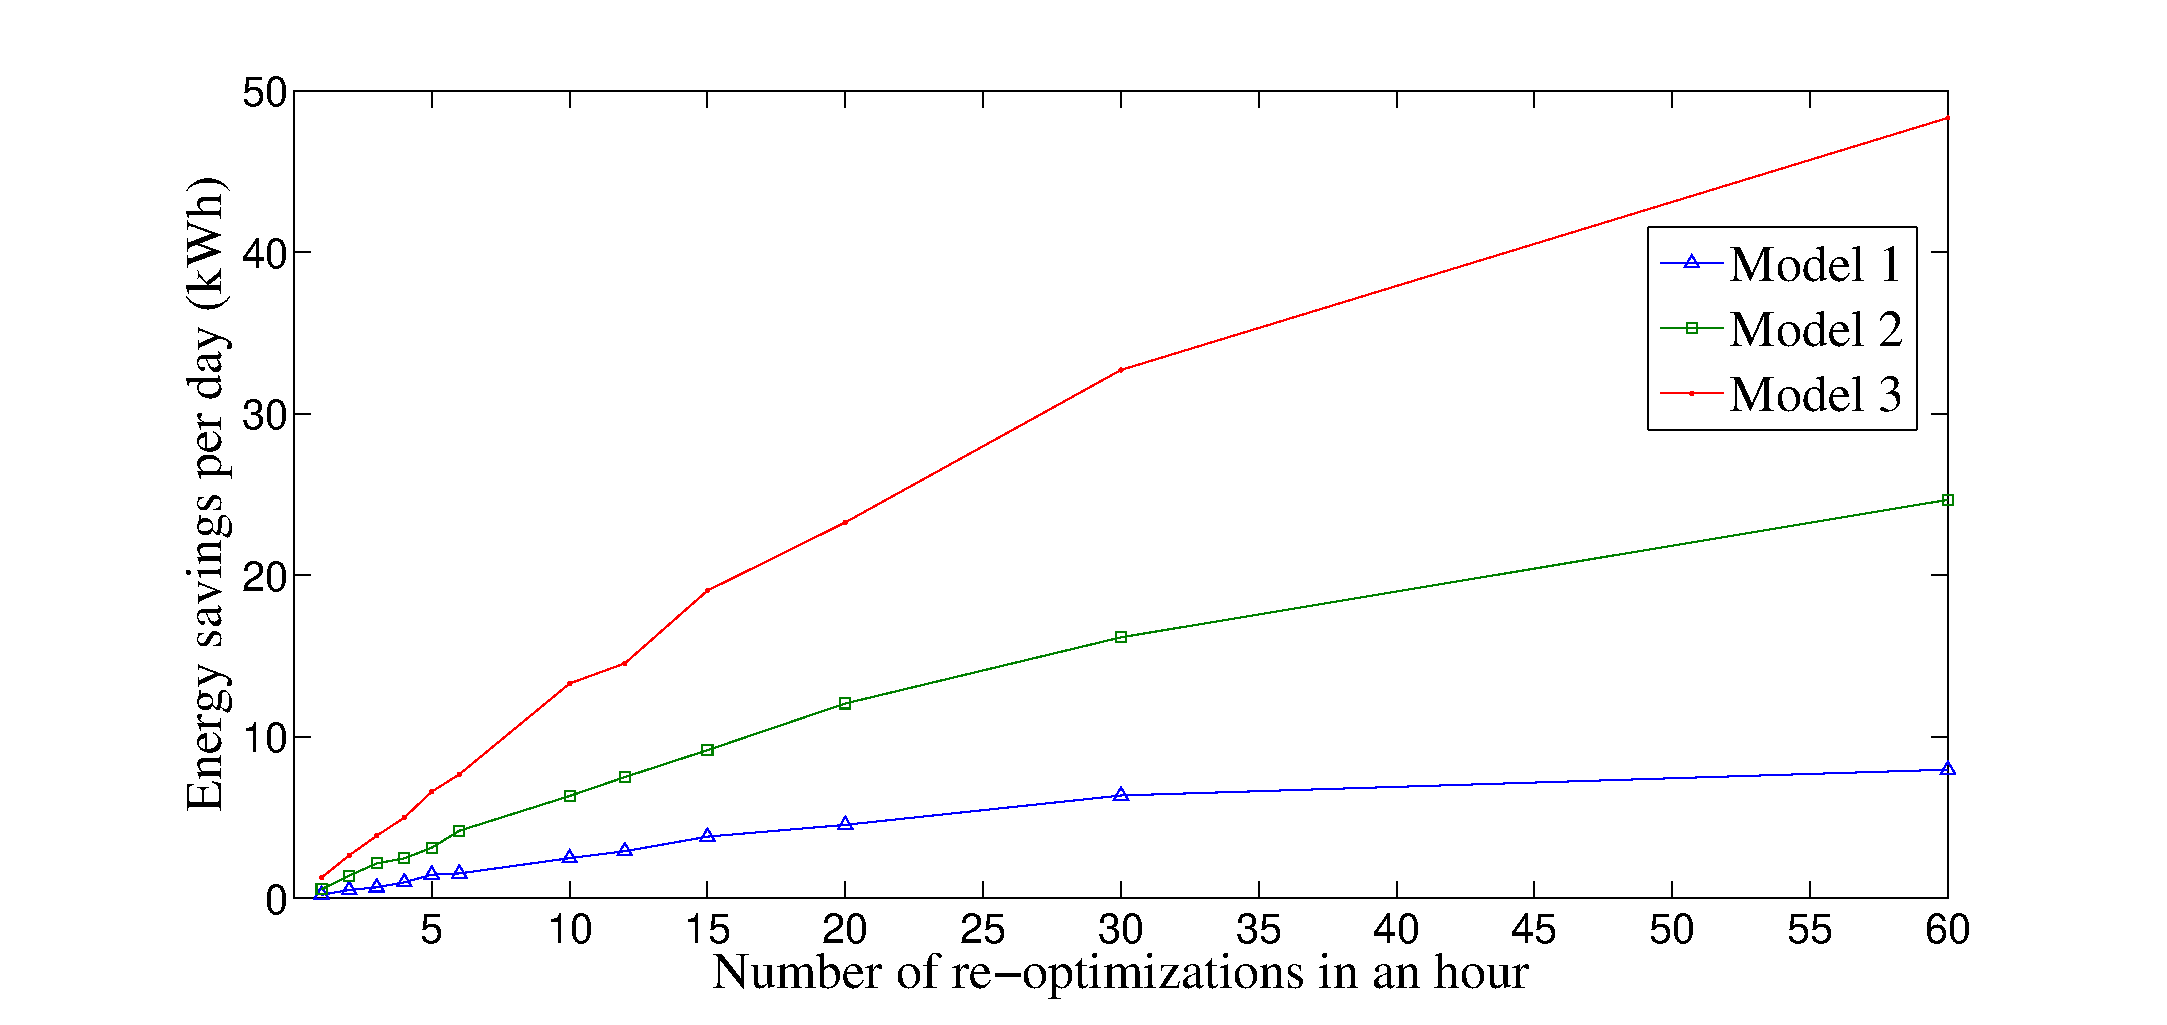
\includegraphics[width=0.5\textwidth]{figures/energysavingssparse.eps}
%\caption{Amount of energy saved per day (kWh) - Sparse deployment of $9$ BTSs}
%\label{fig:results2}
%\end{figure}
%
%We can see the same pattern in the amount of energy saved for the three models as we did for the percentage reduction in power consumption, albeit with model 2 differentiating itself somewhat more clearly from model 1. This is clearly because there is a large difference between the maximum power consumption for model 1 and 2.
%
%One can see in Fig.~\ref{fig:results2} that when re-optimization is done every $5$ minutes, one may be able to save approximately $2.5kWh$, $7kWh$ and $15kWh$ respectively with model 1, 2 and 3. This saving is achieved over a set of $9$ BTSs. In order to understand what kind of savings this translates into for an operator in a country like Pakistan, consider that for an operator named Telenor that has over $7000$ sites in Pakistan~\cite{telenorsitecount} $1800MHz$ band, our results approximate a daily saving of $105MWh$.
%
%For a dense deployment of $9$ BTSs, results of the same set of experiments are plotted in Fig.~\ref{fig:results3} and Fig.~\ref{fig:results4}. These graphs show the same trends as observed for the sparse deployment but with greater magnitudes. For a dense deployment, for instance, when optimizing every $5$ minutes, the savings afforded in a dense deployment for model 3 were about $10kWh$ per day.
%
%\begin{figure}
%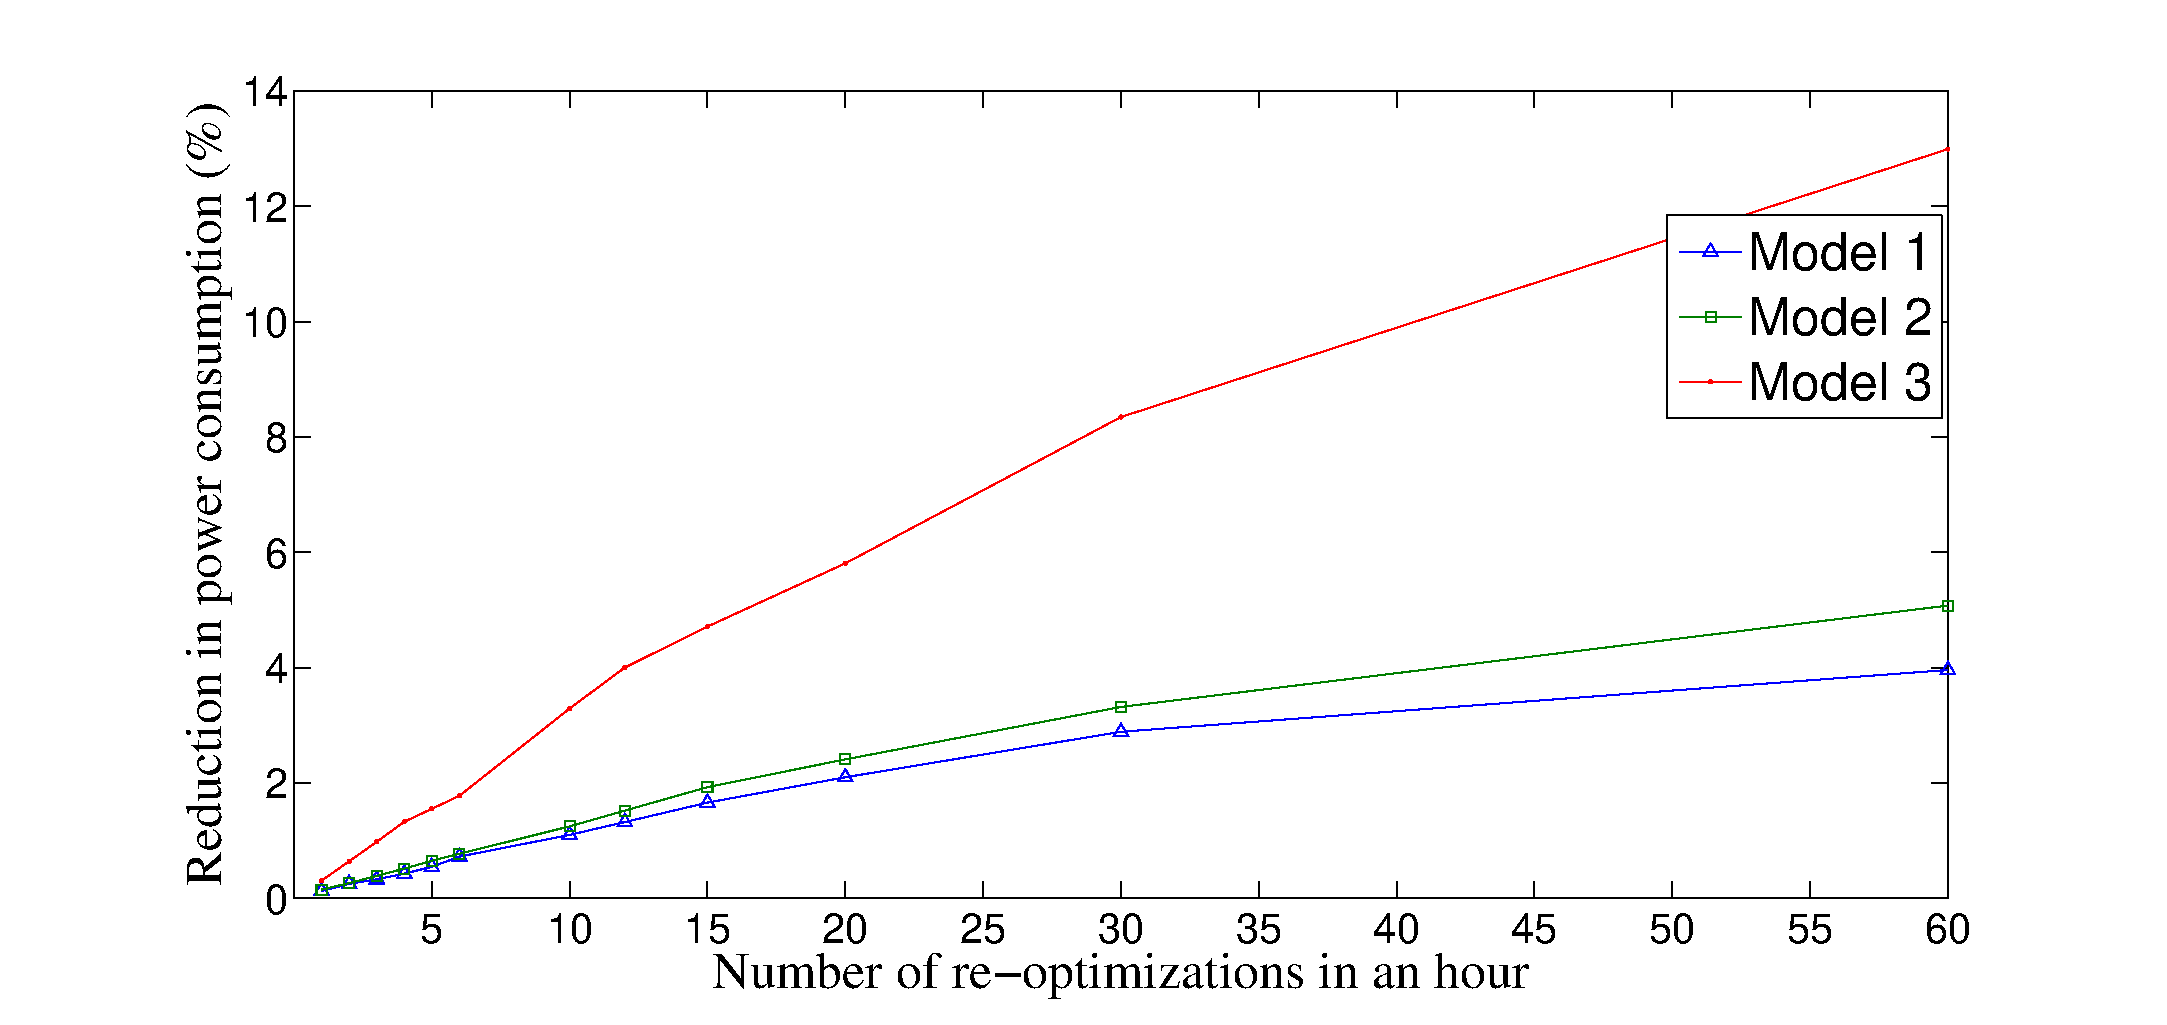
\includegraphics[width=0.5\textwidth]{figures/improvementplotdense.eps}
%\caption{Percentage reduction in power consumption vs re-optimization interval - Dense deployment of $9$ BTSs}
%\label{fig:results3}
%\end{figure}
%
%\begin{figure}
%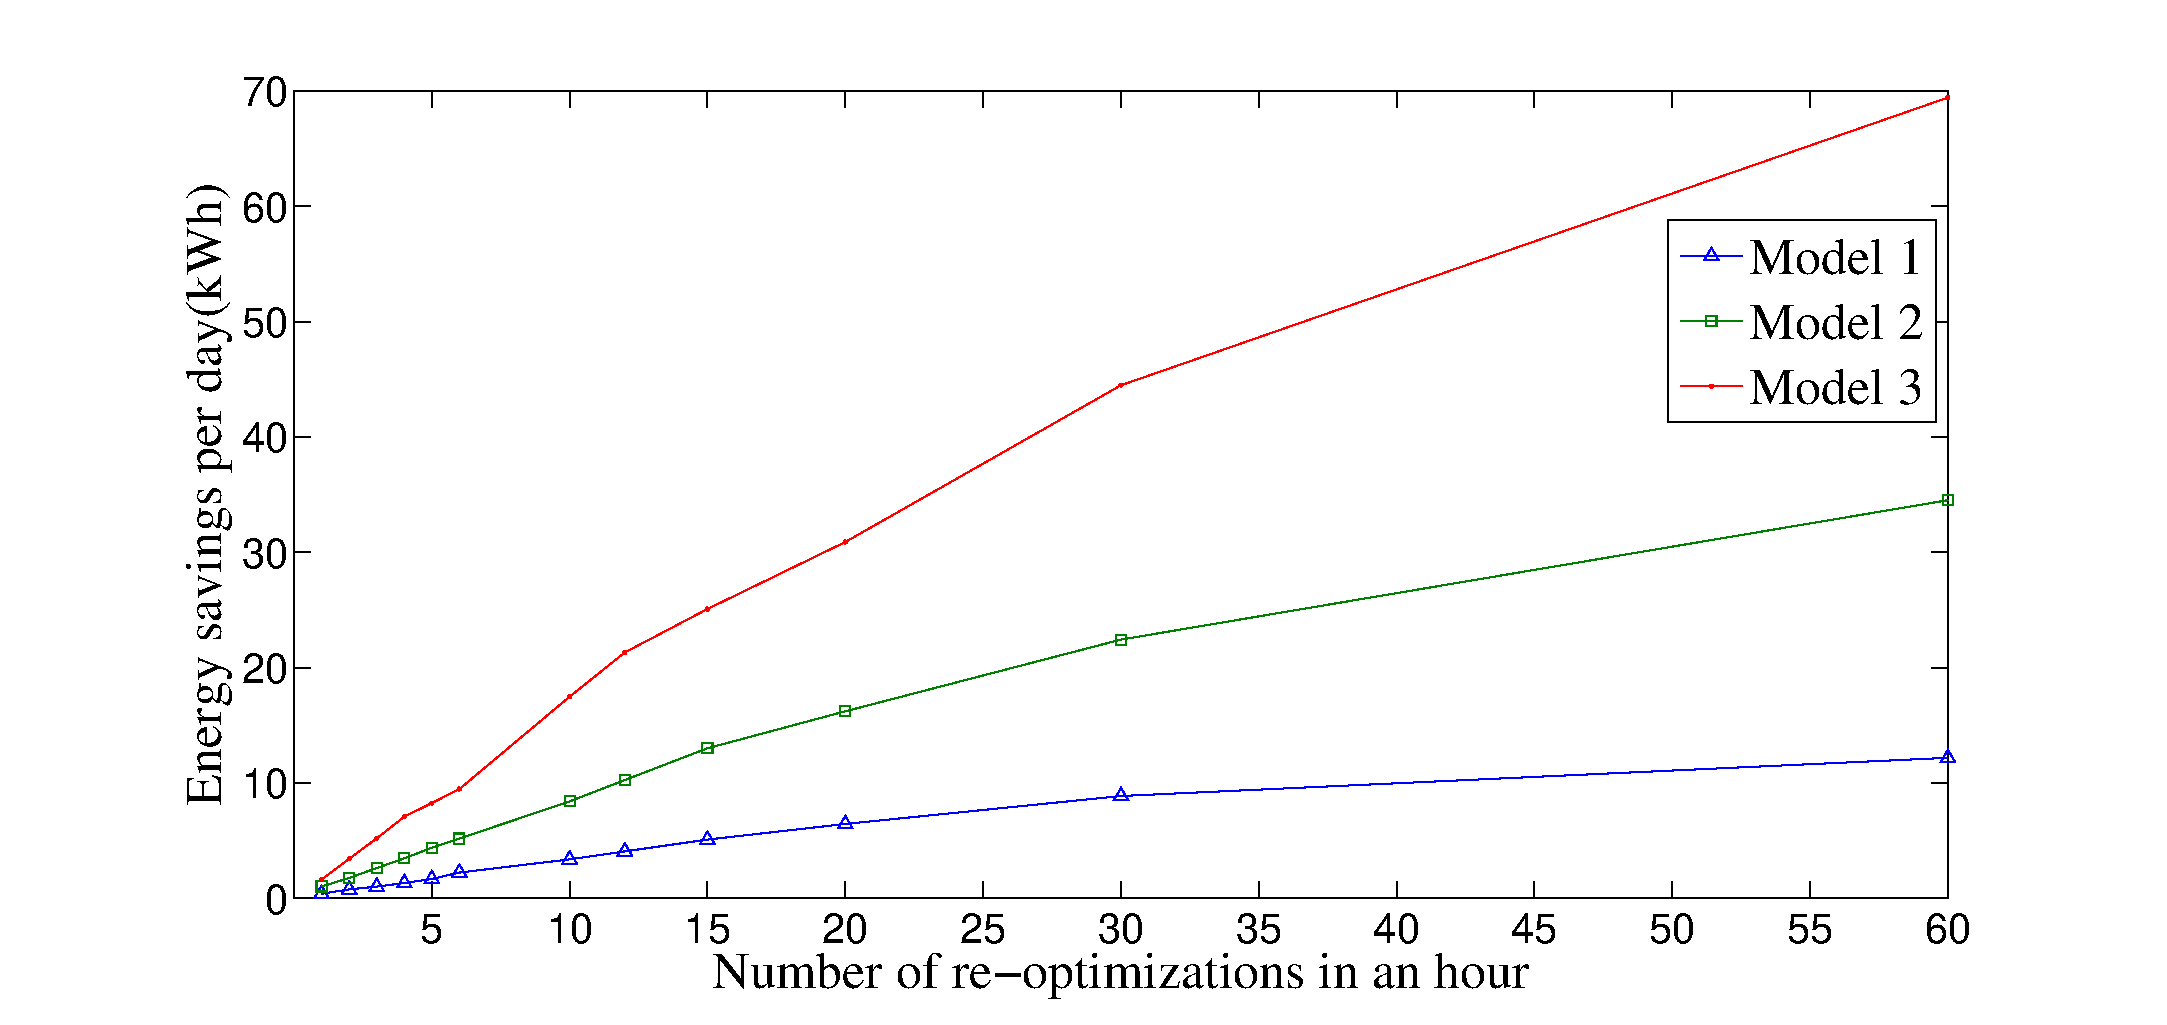
\includegraphics[width=0.5\textwidth]{figures/energysavingsdense.eps}
%\caption{Amount of energy saved per day (kWh) - Dense deployment of $9$ BTSs}
%\label{fig:results4}
%\end{figure}
%
%An operator's network is typically a mix of sparse and dense deployments depending on the spread of subscriber density in their coverage area. For a range of sparse/dense deployment mixes, we computed the approximate achievable reduction in annual energy consumption using the proposed technique. This calculation is just a weighted average of the energy consumption reduction for the sparse and dense deployment as obtained in our experiments. To conserve space, we are listing results only for the case when re-optimization is done every $5$ minutes. The results are listed in table~\ref{tab:benefits}.
%
%\begin{table*}
%\centering
%\begin{tabular}{|c|c|c|c|c|c|c|c|c|c|}
%\hline BTS Model & \multicolumn{9}{|c|}{Sparse/Dense deployment mix (percentages)}\\
%\cline{2-10} \ & 10/90 & 20/80 & 30/70 & 40/60 & 50/50 & 60/40 & 70/30 & 80/20 & 90/10\\
%\hline 1 & 27.58 &	26.77 &	25.97 & 25.16 & 24.35 &	23.55 &	22.74 &	21.94 &	21.13 \\
%\hline 2 & 69.81	& 67.88	& 65.96	& 64.04	& 62.12	& 60.19	& 58.28 & 56.35	& 54.43 \\
%\hline 3 & 144.39 & 139.66	& 134.93	& 130.19	& 125.45	& 120.72	& 115.98	& 111.24	& 106.51
% \\
%\hline
%\end{tabular}
%\caption{Estimated annual energy savings (MWh) for $7000$ sites in \\ various mixes of sparse and dense deployment}
%\label{tab:benefits}
%\end{table*}

%It is important to consider the cost of this scheme if it is to be deployed in practice. On average, each re-optimization took an average of about one minute when run on a laptop computer with a Core i3 processor and 4 GB of RAM, for the 26 BTS dataset that we considered. Further improvements in running time alongwith joint optimization of a greater number of sites simultaneously can be achieved through a more powerful computer and/or parallelization. However, BIP is an NP-Hard problem, so expecting to solve an online optimization of traffic over a city's entire network would be unrealistic. We must, therefore, come up with heuristics to solve this problem sub-optimally. One heuristic, as proposed in this paper is to separately optimize traffic over small sets of BTSs. Other approaches such as approximations to similar classes of problems (such as the assignment problem) and evolutionary algorithms need to be tried and will be explored in an extended version of this paper.
\section{Conclusions}
\label{sec:conclusions}
BTSs account for most of a cellular network's energy consumption. Motivated by the non load-proportionality of BTS energy consumption, prior work proposed shutting down some BTSs when traffic is low. However, network operators are reluctant to do so for a variety of reasons.

To reduce energy consumption, we propose using a commonly available and used feature called BTS power savings that deactivates some TRXs at BTSs that have low traffic. Furthermore, calls may be handed-off from BTSs with higher load to neighboring ones with lighter load to increase the benefits of BTS power-saving.

Using real network topology and traffic traces in a simulation study , we found that merely using BTS power saving in an urban setting can result in considerable energy savings. Moreover, our results also indicate that periodic call-shuffling between BTSs can further reduce energy consumption in existing large GSM networks.
%% The Appendices part is started with the command \appendix;
%% appendix sections are then done as normal sections
%% \appendix

%% \section{}
%% \label{}

%% References
%%
%% Following citation commands can be used in the body text:
%% Usage of \cite is as follows:
%%   \cite{key}         ==>>  [#]
%%   \cite[chap. 2]{key} ==>> [#, chap. 2]
%%

%% References with bibTeX database:

\bibliographystyle{elsarticle-num}
\bibliography{ref}

%% Authors are advised to submit their bibtex database files. They are
%% requested to list a bibtex style file in the manuscript if they do
%% not want to use elsarticle-num.bst.

%% References without bibTeX database:

% \begin{thebibliography}{00}

%% \bibitem must have the following form:
%%   \bibitem{key}...
%%

% \bibitem{}

% \end{thebibliography}


\end{document}
